\chapter{État final de développement}

L'avancement actuel du projet, permet : 
\begin{itemize}
	\item d'établir une connexion Ethernet entre le PC hôte et la liseuse
	\item de modifier l'affichage de l'écran E-Ink
\end{itemize}

La mise en place de la connexion Ethernet se fait grâce aux modifications effectuées sur le système de fichier monté par la liseuse.

% 1 : l'image de la liseuse
%ethernet
	%connection de l'interface reseau eth1 
\section{Fonctionnalités de l'image} %a changer

\subsection{La connexion Ethernet}
La liseuse ne disposant que d'un port USB il faut passer par un module chargeable pour émuler une connexion Ethernet sur ce port.
Ce module est le gadget Ethernet d'Android.
Le réseau établi entre la liseuse et le PC est défini statiquement, de plus les adresses MAC des cartes émulées sont fixées par le module.

%capture d'ecran ifconfig
\begin{figure}[]
	\begin{center}
	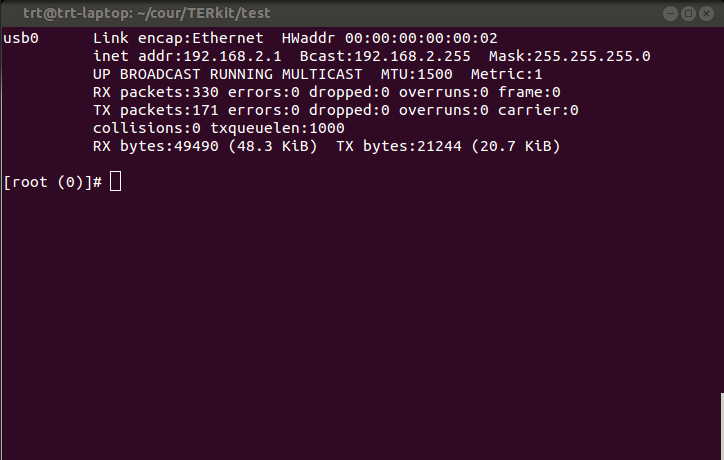
\includegraphics[scale=0.5]{capt_prs_ifconfig.png}	
	\end{center}
	\caption{Configuration réseau de la liseuse}
\end{figure}

\begin{figure}[]
	\begin{center}
		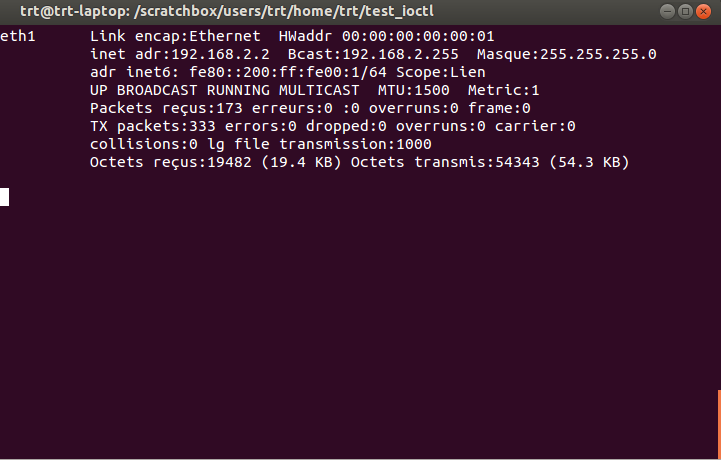
\includegraphics[scale=0.5]{capt_pc_ifconfig.png}
	\end{center}
	\caption{configuration réseau du PC}
\end{figure}
\clearpage
%dropbear
\subsection{L'ajout de dropbear}
Pour des raisons pratiques nous avons ajouté à la liseuse la gestion du protocole SSH, afin de pouvoir lancer facilement des commandes sur la liseuse, mais aussi de faciliter la copie de fichiers.
%a voir ci c'est util
L'utilisation de dropbear est pratiquement identique à celle du SSH que l'on peut trouver sur un système Linux. De légères différences subsistes si une connexion en SSH de la liseuse au PC hôte car les commandes ne sont pas nommées comme sur un système classique. Pour démarrer le serveur Dropbear (SSH) la commande est la suivante : 

\begin{lstlisting}
dropbear start
\end{lstlisting}

Normalement dropbear est démarré au lancement de la Liseuse en mode Recovery. De plus si une connection ssh veut être initialisé de la liseuse, il faut lancer la commande suivante :

\begin{lstlisting}
dhclient [nom-hote]@[IP-hote]
\end{lstlisting}



\section{Programme d'affichage}

La modification de l'écran E-Ink peut se faire de deux manières, soit en envoyant les commandes directement au driver (en utilisant les ioctl), soit en passant par une librairie graphique (ici DirectFB).

\subsection{Affichage via ioctl}

Le programme de test d'affichage via ioctl permet d'envoyer un buffer d'affichage directement dans le framebuffer du driver EPDC.
Ici ce buffer est constitué de pixels aléatoire : 
%capture d'écran get_temp
	
	\begin{figure}[h!]
		\begin{center}
			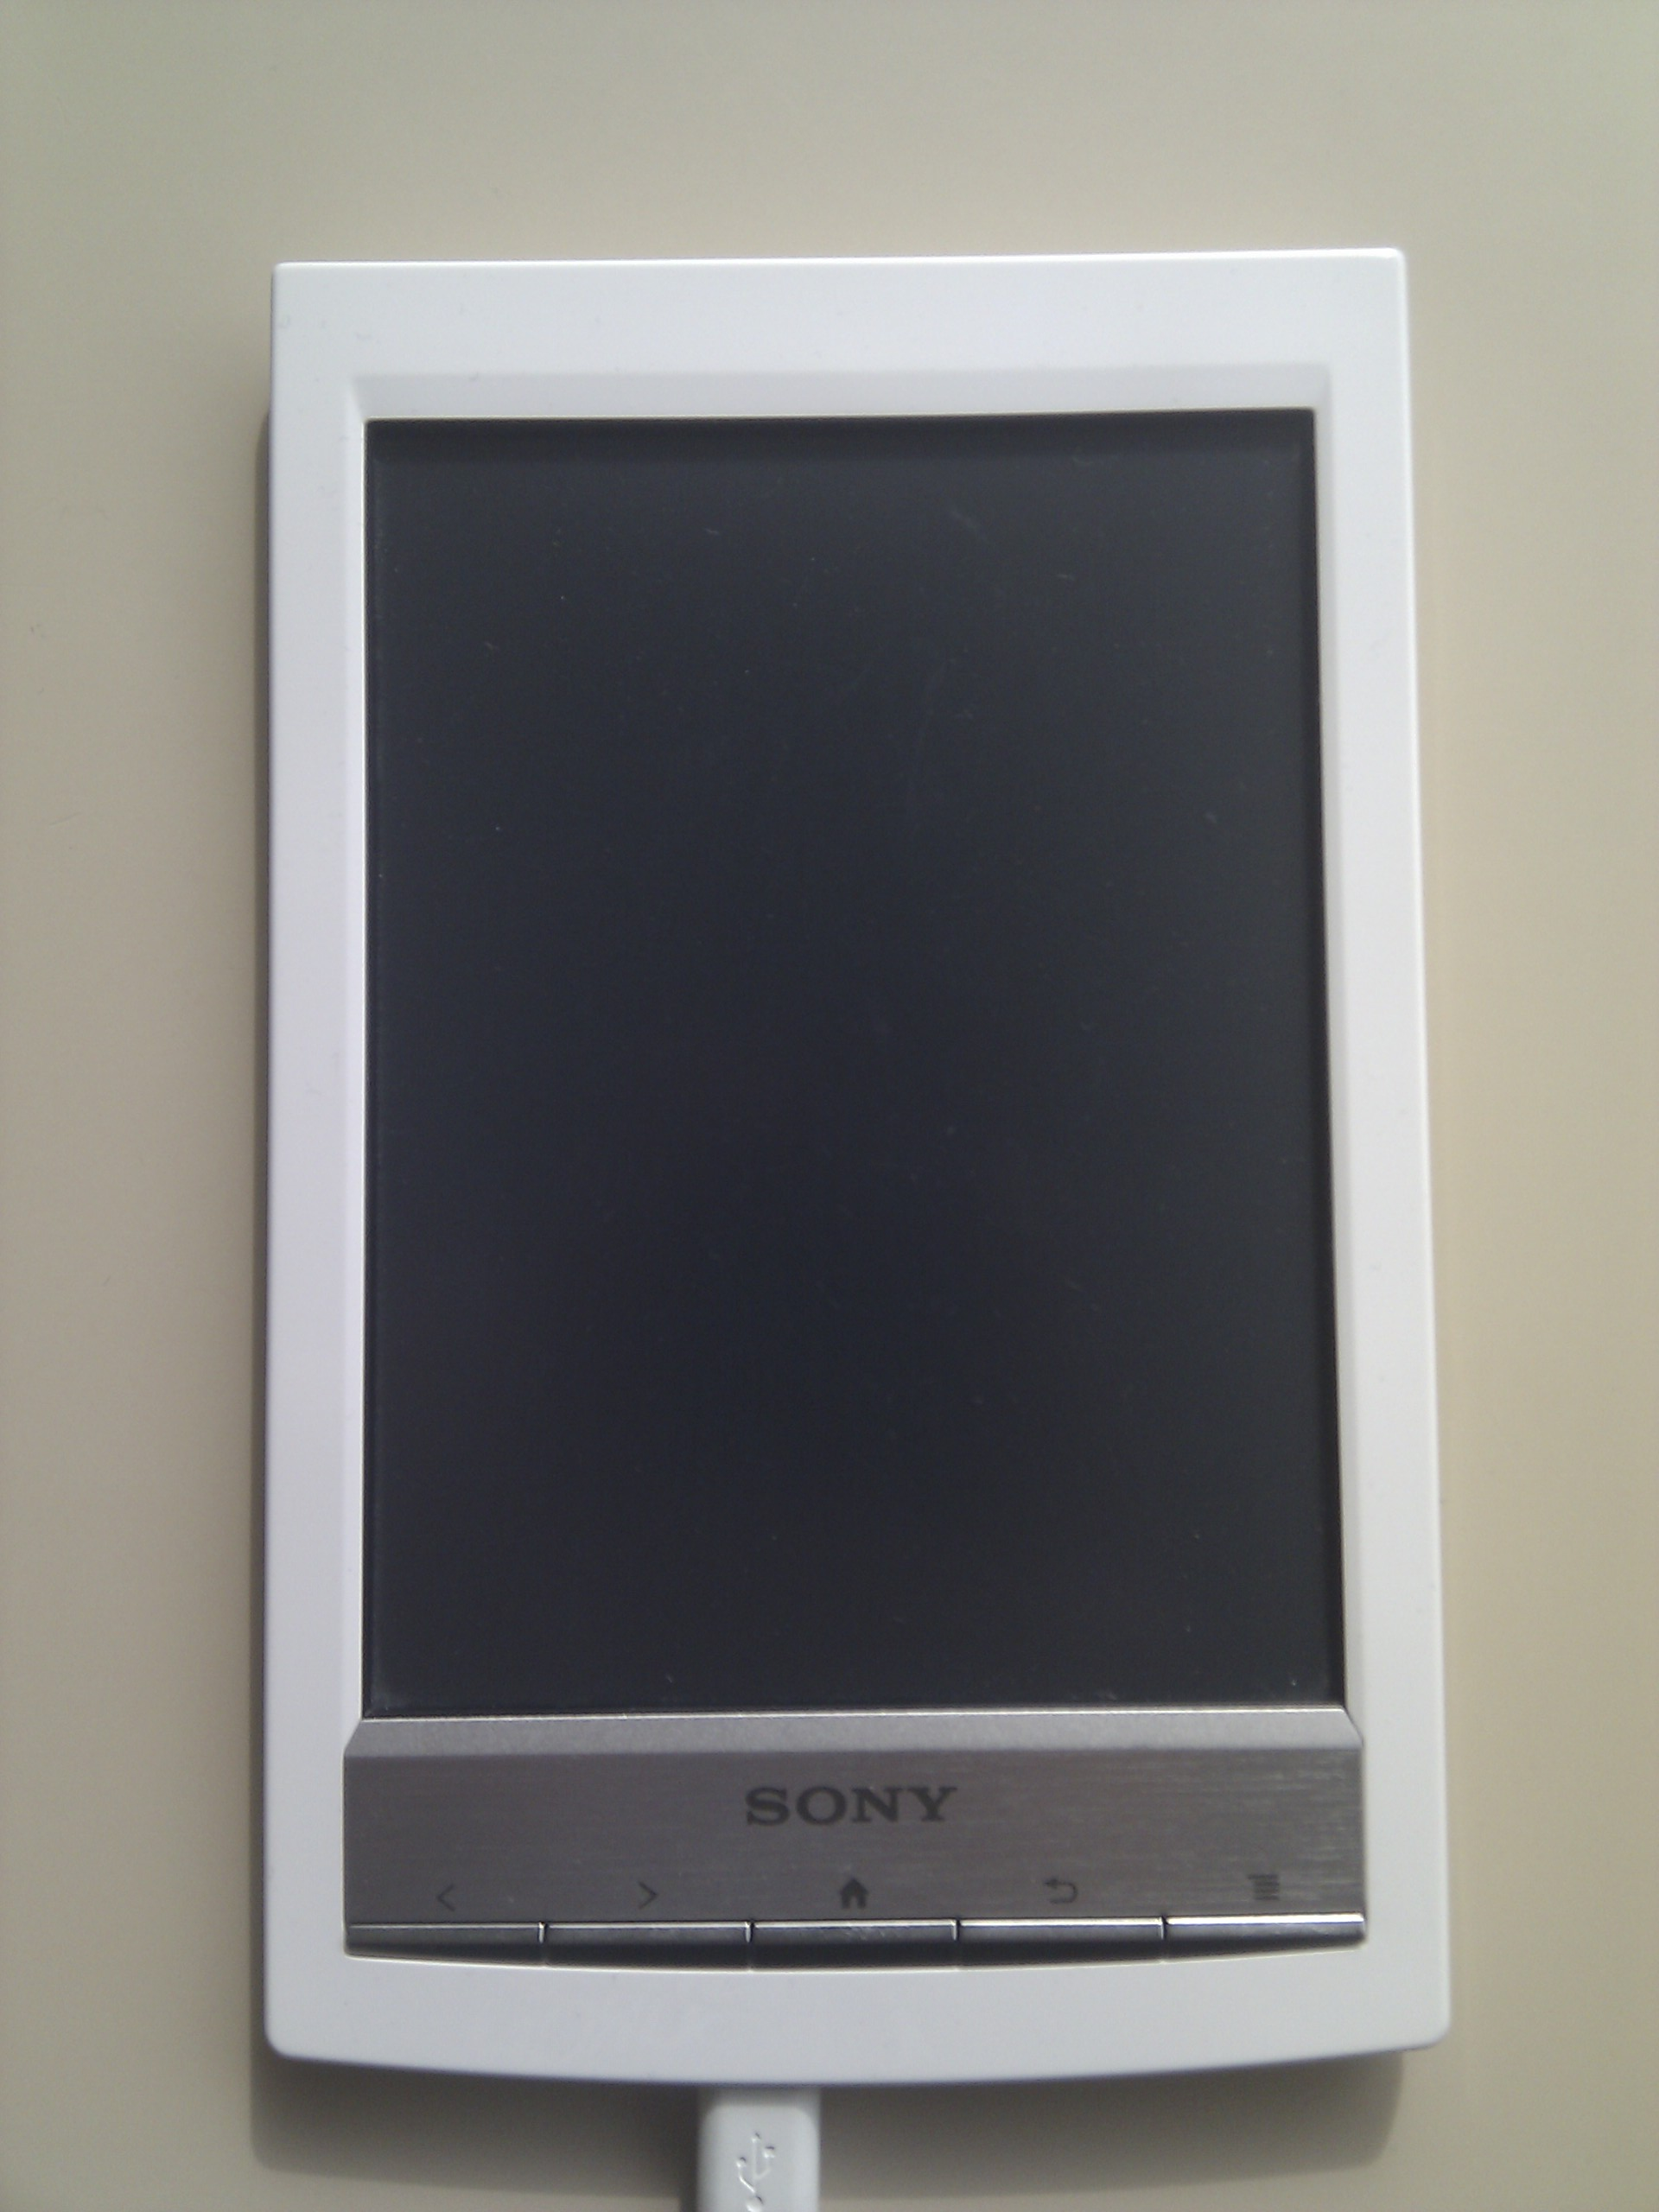
\includegraphics[scale=0.15]{screen_get_temp.jpg}
			 \caption{Modification de l'affichage en utilisant les ioctl}
		\end{center}
	\end{figure}
\subsection{Affichage via DirectFB}

Le programme d'affichage via Librairie graphique génère le framebuffer en utilisant les primitives de DirectFB.
Le programme de test dessine ici 10 lignes avec points d'arrivé aléatoire.

	\begin{figure}[h!]
		\begin{center}
			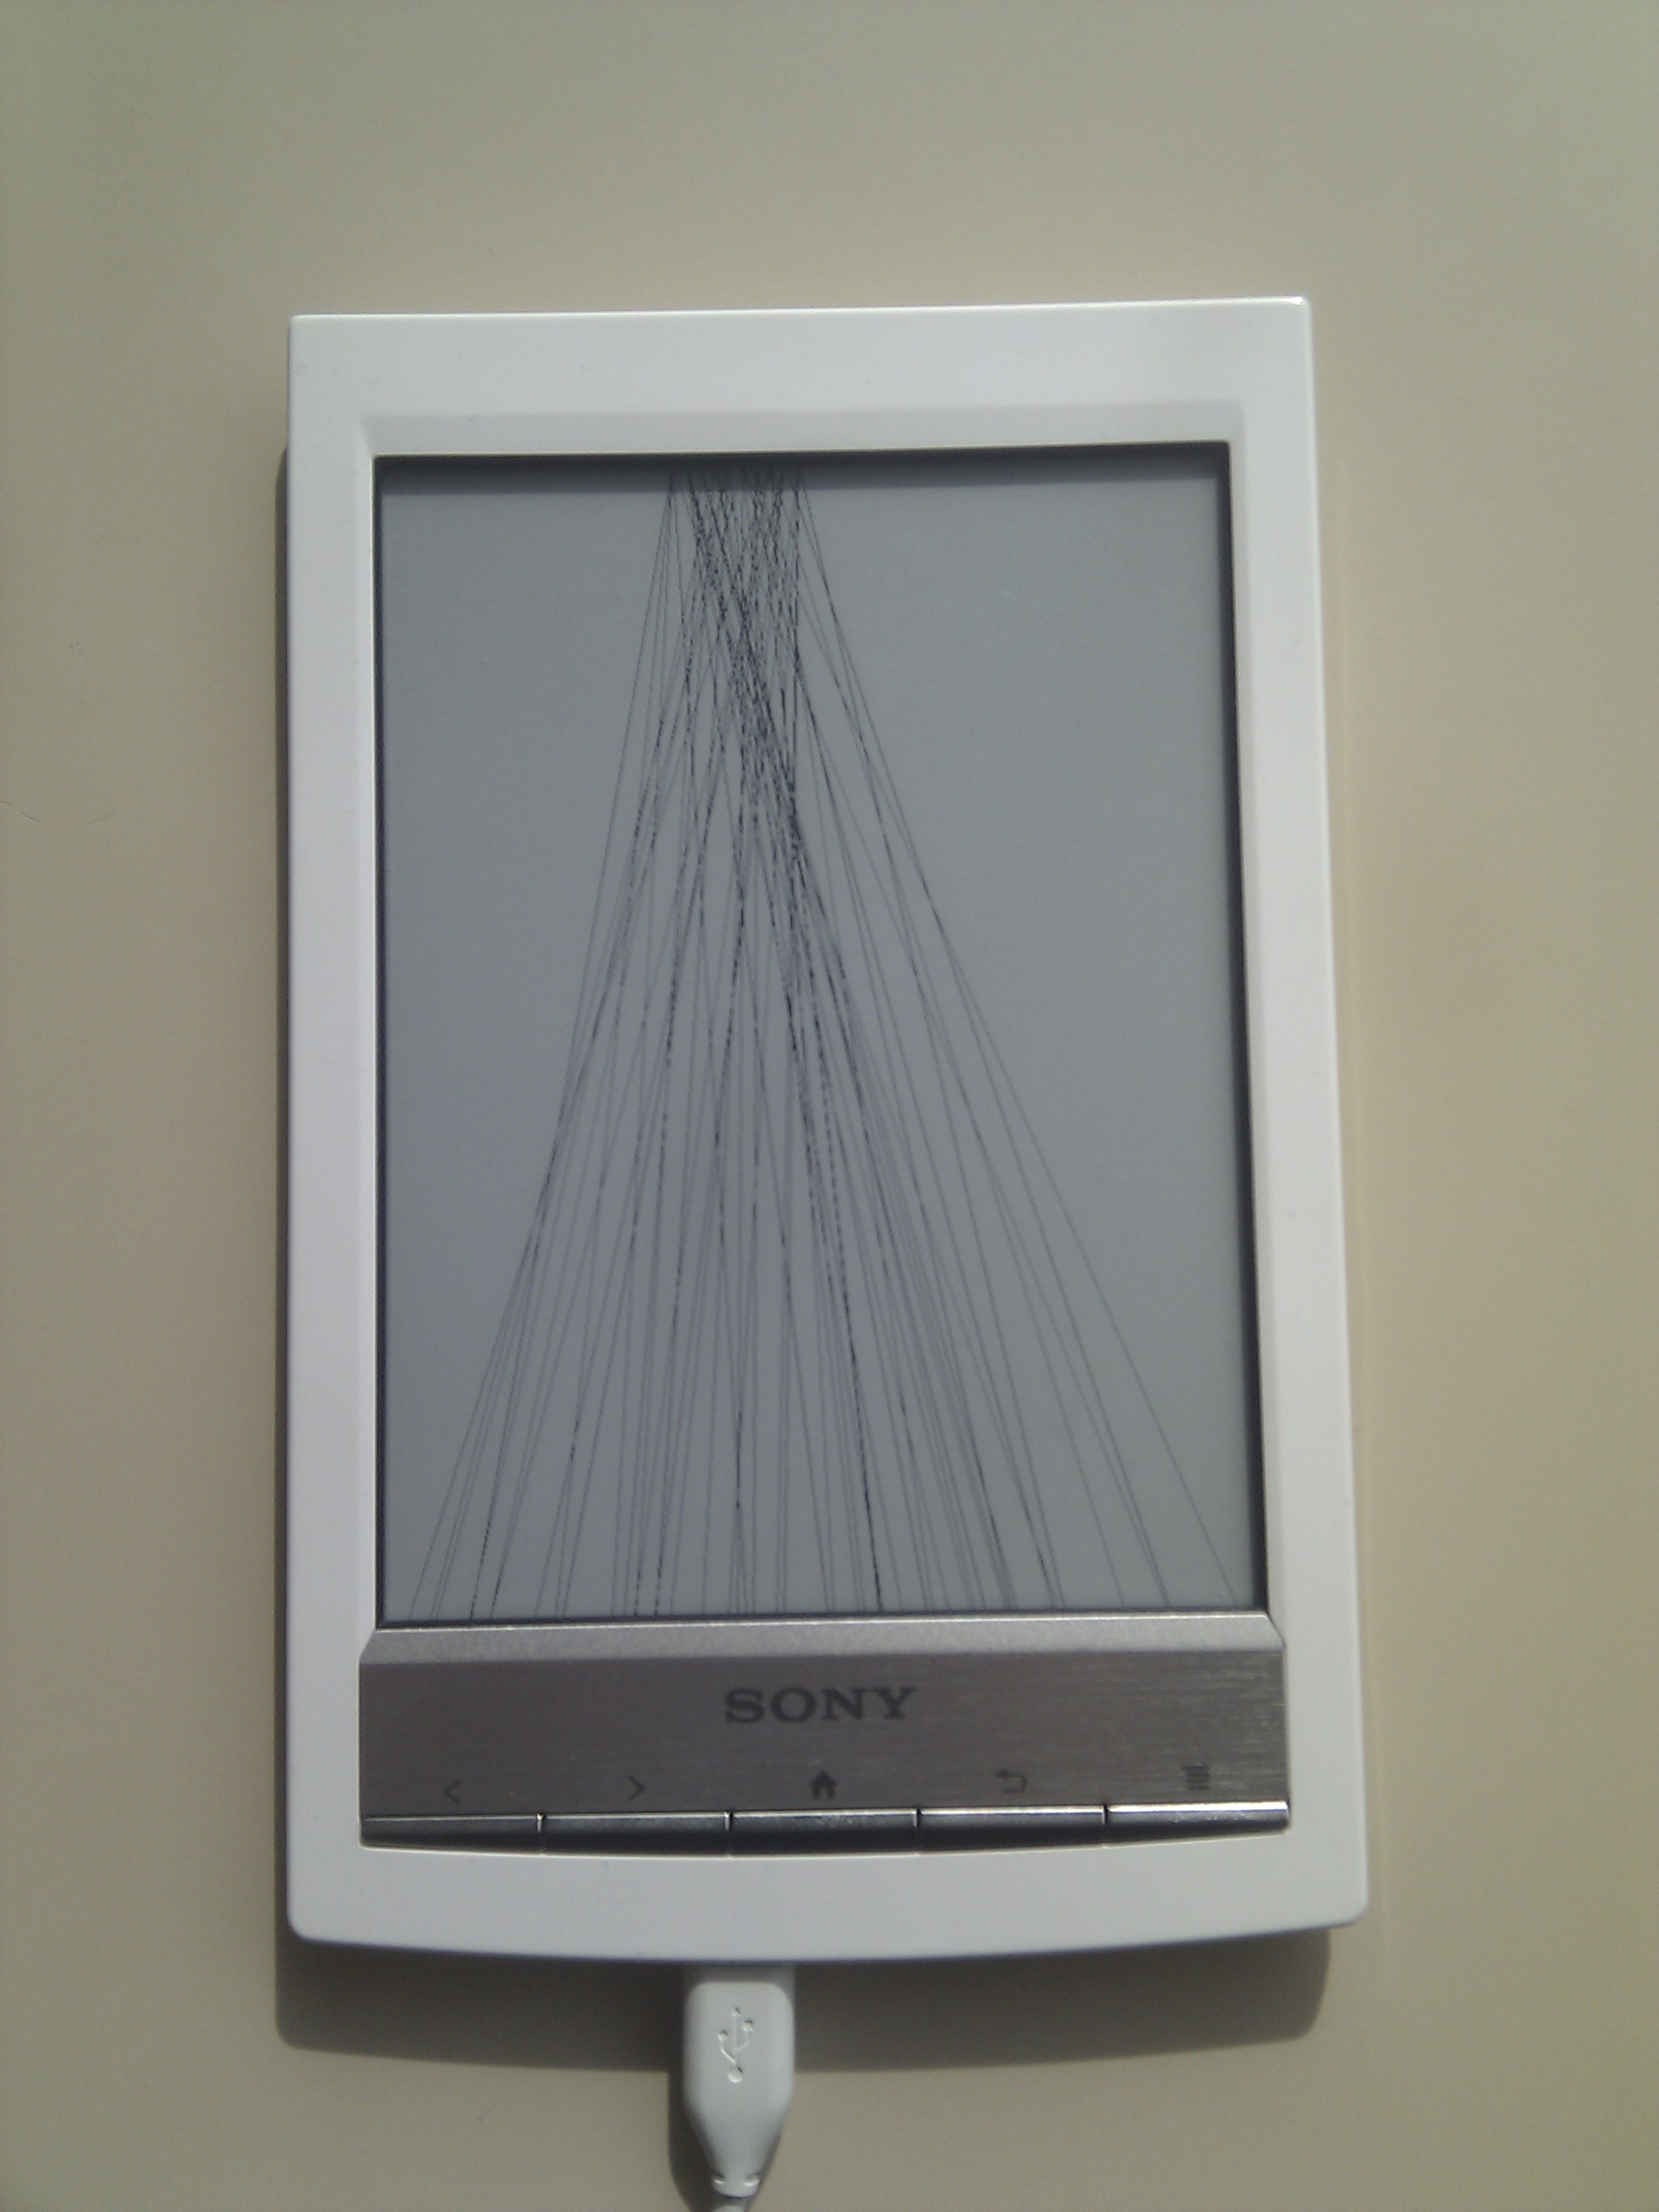
\includegraphics[scale=0.15]{screen_direct.jpg}
			\caption{modification de l'affichage en utilisant DirectFB}
		\end{center}
	\end{figure}

%capture direct
% 2 : programme d'affichage
%exemple de fonctionnement
